
\documentclass[twocolumn,showpacs,superscriptaddress,groupedaddress]{revtex4}
\usepackage{graphicx}
\usepackage{dcolumn}
\usepackage{bm}  
\usepackage{amssymb}  
\usepackage{hyperref}
\hypersetup{colorlinks=true, urlcolor=blue, citecolor=blue}


\begin{document}


\title{\vspace{-15mm}\fontsize{24pt}{10pt}\selectfont\textbf{A Radial Time 
Projection Chamber for $\alpha$ detection in CLAS at JLab}}
\input author_list.tex  

\date{\today}

\begin{abstract}
A new Radial Time Projection Chamber (RTPC) was developed at Jefferson 
Laboratory to track low-energy nuclear recoils for the purpose of measuring
exclusive nuclear channels, such as coherent Deeply Virtual Compton Scattering
and coherent meson production on $^4$He. In such processes, the $^4$He nucleus
remains intact and recoils as a whole in the final state. The CEBAF Large
Acceptance Spectrometer (CLAS) has been used for similar studies on proton
targets, however it cannot track low energy $\alpha$ particles. In
2009, we carried out measurements using the CLAS spectrometer supplemented by
the RTPC positioned directly around a gaseous $^4$He target, allowing a detection
threshold as low as $~$150  MeV/c for $^4$He. This article discuses the design,
work principle, calibration methods and performances of the RTPC.
\end{abstract}

\maketitle

\section{Introduction} \label{sec:level1}

Thomas Jefferson National Accelerator Facility (TJNAF), in Newport News, Virginia,
USA, provides high power electron beams of energy up to 6 GeV and 100$\%$ duty cycle
to three experimental Halls (A, B, C) simultaneously. The CLAS spectrometer, located
in Hall-B, is composed of several sub-detectors and two magnets. The spectrometer
was designed to track charged particles of momentum greater than 250 MeV/c as well 
as detecting real photons. Figure~\ref{fig:CLAS} shows a three dimensional 
representation of the baseline CLAS spectrometer:
\begin{itemize}
 \item Three regions of Drift Chambers (DC) for the tracking of charged 
    particles~\cite{DCref} (in blue on the figure).
 \item Superconducting toroidal magnet (in yellow) to bend the trajectories 
    of charged particles, thus allowing momentum measurement with the DC tracking information.
 \item Cherenvkov Counters (CC) to distinguish electrons from other negative 
    particles, such as pions, at lower energies~\cite{CCref} (in pink).
 \item Scintillation Counters (SC) to identify hadrons by measuring their 
    time of flight (TOF)~\cite{TOFref} (in red).
 \item Electromagnetic Calorimeters (EC) to distinguish electrons from other negative 
    particles at higher energies and to detect neutral particles (neutrons and 
    photons in particular)~\cite{ECref} (in green).
\end{itemize}

\begin{figure}[tbp]
\centering 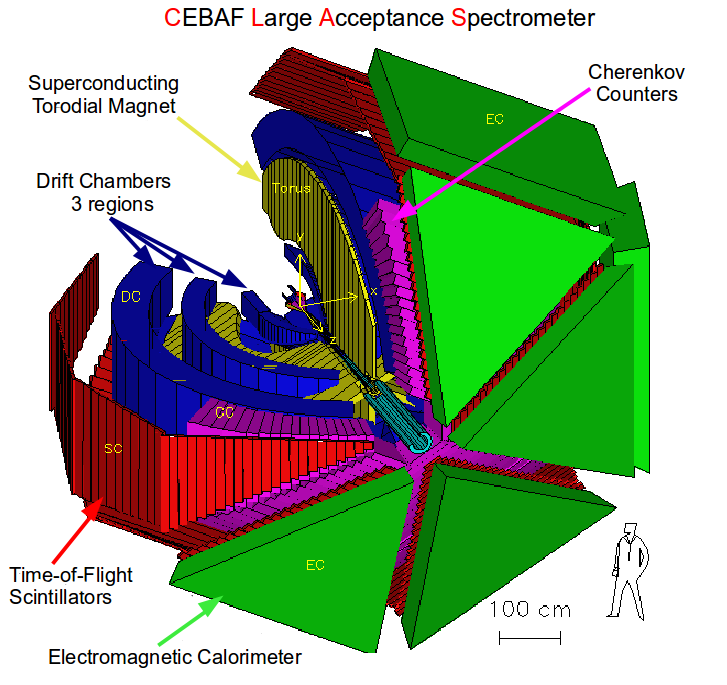
\includegraphics[scale=0.3]{fig/test_clas.png}
\caption{A three dimensional representation of the baseline CLAS setup. The
   full description is given in the text.} \label{fig:CLAS}
\end{figure}

Measurement of the Deeply Virtual Compton Scattering (DVCS) process
($eH \rightarrow e' H' \gamma$, where $H$ is a hadron) necessitates an upgrade
of this setup.  With a 6 GeV electron beam, the majority of DVCS photons are produced
at very forward angles, where the acceptance of the EC is poor. To extend the detection range,
an inner calorimeter (IC) was built for the E01-113 experiment in 2005.
The IC is constructed from 424 lead-tungstate (PbWO$_{4}$) crystals, covering polar 
angles between 5$^{\circ}$ and 15$^{\circ}$. Each crystal is 16 cm long, corresponding
to 17 radiation lengths. The achieved energy resolution is around 3 to 4$\%$ for photon
energies between 2 GeV and 5 GeV, with an angular resolution between 3 and 5 mrad 
\cite{Hyon-suk}. To protect this detector from the large flux of low energy M{\o}ller 
electrons, a 5~T solenoid was placed around the target to shield the IC. 
In addition, the recoil nuclei of the coherent DVCS on helium was detected 
using a RTPC developed to track low energy nuclear fragments. The solenoid field
serving as the analyzing magnet for the particle tracking in the RTPC. This 
setup was used during a three months experimental run
in 2009 with a longitudinally polarized electron beam of 6.064 GeV incident 
on a gaseous $^{4}$He target.
{\bf \color{red} Add beam current or luminosity.}

In this paper we report the design, calibration, and performance of the radial TPC,
organized as follows. Section \ref{sec_design} details the physics considerations for our RTPC's
design and internal structure. Section \ref{sec_readout} describes the properties
of the read-out system. Calibration strategies are discussed in section \ref{sec_calib}.
Finally, the performance of the RTPC is described in section \ref{sec_perf}.


\section{CLAS RTPC design} \label{sec_design}

With a 6 GeV incident electron energy, the recoiling $^{4}$He nuclei from coherent 
DVCS have an average momentum around 250 MeV/c. Such low energy $\alpha$ 
particles are stopped very rapidly, so the RTPC was designed to be as close 
as possible to the target and fitting within the 230~mm diameter 
of the 5 Tesla solenoid magnet surrounding the target \cite{Hyon-suk}. 

\begin{figure}[tb]
\centering
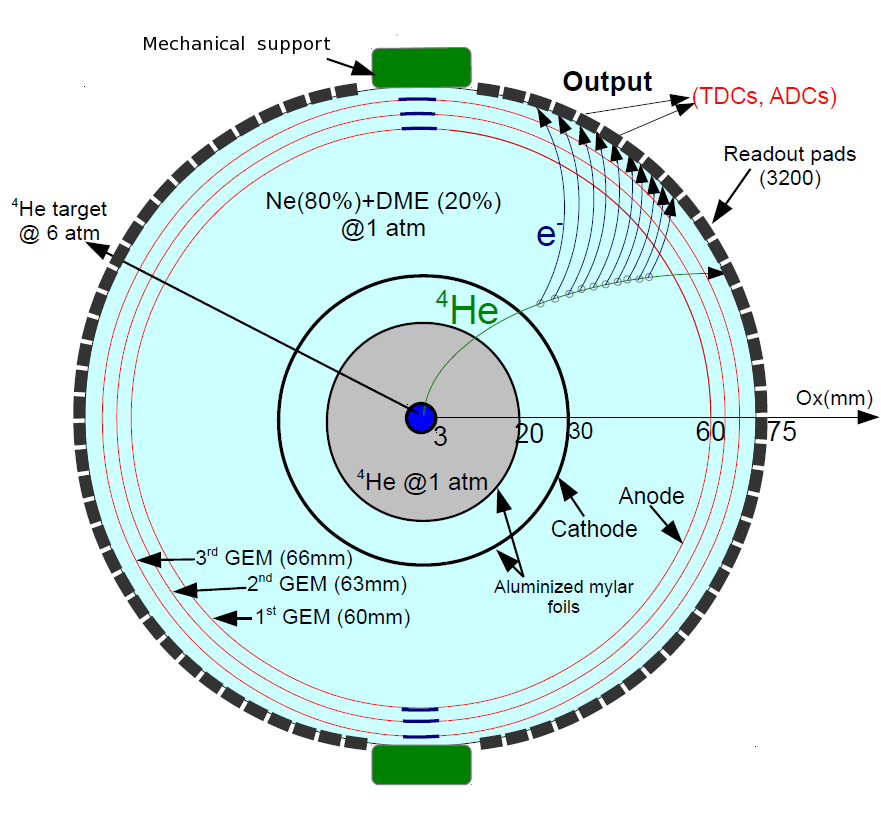
\includegraphics[scale=0.28]{fig/RTPC_1_all.png}
\caption{Schematic drawing of CLAS RTPC in a plane perpendicular to 
the beam direction.  See text for description of the elements.} 
\label{fig:RTPC_1_4}
\end{figure} 

The CLAS RTPC is a 250~mm long cylinder of 158~mm diameter, leaving just enough 
room to fit pre-amplifiers between the RTPC outer shell and the solenoid. The 
electromagnetic field is directed perpendicularly to the beam direction, 
such that drifting electrons are pushed away from the beam line. These electrons 
are amplified by three layers of curved GEMs and detected by the readout system 
on the external shell of the detector as illustrated in the figure~\ref{fig:RTPC_1_4}. The CLAS 
RTPC is segmented into two halves with independent GEM amplification systems that 
cover about 80\% of the azimuthal angle.

We detail here the different regions shown in figure~\ref{fig:RTPC_1_4} starting 
from the beam line and towards larger radius:\\
\begin{itemize}
   \item First, the 6 atm helium-4 target extends along the beam line axis, it 
      is 284~mm long with a 3~mm radius wall made of a 27-$\mu$m-thick Kapton.
   \item The first gas gap covers a radial range from 3 mm to 20 mm. It is 
      filled with $^{4}$He gas at 1~atm to minimize secondary interactions from
      M\o ller electrons scattered by the beam. This 
      region is surrounded by a 4 $\mu$m thick window made of aluminized Mylar 
      and electronically grounded.
   \item The second gap region extends between 20~mm and 30~mm and is filled with a 
      gas mixture of 80$\%$ Neon and 20$\%$ Dimethyl Ether (DME). This region 
      is surrounded by a 4~$\mu$m thick window made of aluminized Mylar, which 
      serves as the cathode. {\bf \color{red} What Voltage ?}
   \item The drift region is filled with the same Ne-DME gas mixture and extends 
      from the cathode to the first Gas Electron Multiplier(GEM), 60 mm away 
      from the beam axis. The electric field in this region is around 500~V/cm 
      {\bf \color{red} Give exact value.} and perpendicular to the beam.
   \item The electron amplification system is composed of three GEMs located at 
      radii of 60, 63 and 66 mm. In this configuration, the first GEM layer 
      represents the anode. {\bf \color{red} What bias voltage ?}
   \item The readout board has an internal radius of 69~mm and collects charge
     from the GEMs. Preamplifiers are plugged directly on its outer side and
     transmit the signal to the data acquisition electronics.
\end{itemize}

\begin{figure}[tbp]
\centering
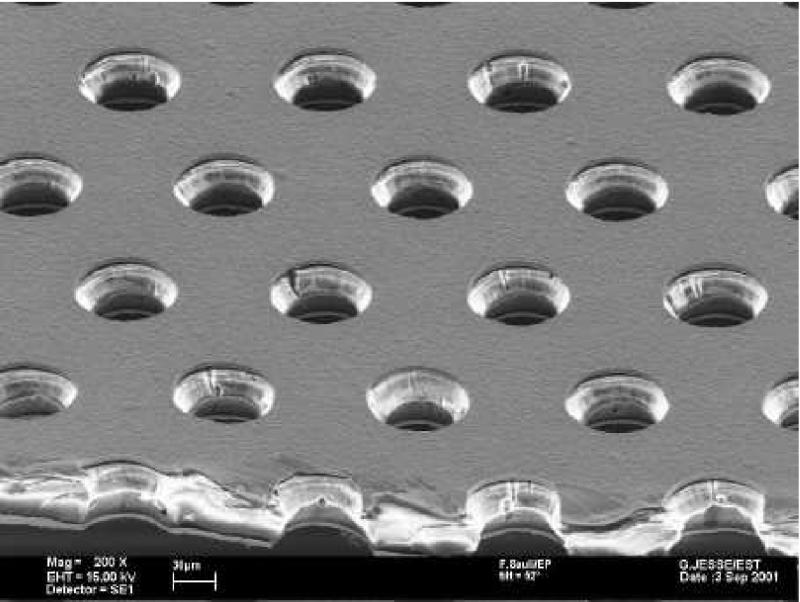
\includegraphics[scale=0.70]{fig/GEM_photo.jpg}
\caption{Picture of a GEM foil similar to the one used for our RTPC.} 
\label{fig:GEMs}
\end{figure}

The GEM technology has been chosen for this RTPC for its flexibility, 
allowing a curved amplification surface. Also, GEMs are known to rarely create 
sparks{\bf \color{red} Need reference.}, which is important when trying to 
detect highly ionizing slow nuclei that deposit large amount of energy. The 
GEMs for this RTPC are made from a Kapton insulator layer 
{\bf \color{red} Thickness?} sandwiched between two 5 $\mu$m copper
layers. The mesh of each GEM layer is chemically etched with 50$\mu$m diameter
holes with double-conical shapes as illustrated in figure~\ref{fig:GEMs}. A
potential difference of 400 V {\bf \color{red} To be checked and set as above.} 
is applied between the two copper layers of the
GEM, creating a very strong electric field in each hole leading to high ionization 
and therefore amplification of the incoming electrons. A 
potential of 150 V {\bf \color{red} To be checked.} 
is set between the GEMs to push the electrons toward the next GEM and eventually 
the readout pads. The gain of each GEM layer is of order 100, making a total gain 
of about $10^{6}$. {\bf \color{red} We should quote a realistic overall gain or nothing.}\\

{\bf \color{red} To be added:

Discuss the choice of drift gas

Discuss the self supporting mechanic of the GEMs.}

\section{Readout System} \label{sec_readout}

\begin{figure}[tb]
   \centering
   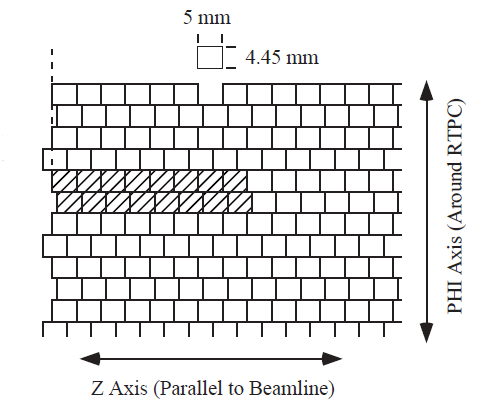
\includegraphics[scale=0.55]{fig/PADs.png}
   \caption[]{A schematic representation of a part of the readout system.  The 
   shaded sixteen pads are a group of pads that are connected to the same 
pre-amplifier.} \label{fig:PADs}
\end{figure}

The RTPC electron collection system has 3200 readout pads. These elements are
located at the end of the amplification region, 69 mm from the central axis.
Figure \ref{fig:PADs} shows a schematic drawing of the size and 
configuration of the pads. Each readout pad is 5 mm in length and 4.45 mm in 
width.  The shift between the rows allows to reduce aliasing. Each half of the 
RTPC has 40 rows and 40 columns of pads. The shaded region in figure~\ref{fig:PADs}
shows how pads are grouped to 16 channels pre-amplifiers.  A Time to Digital
Converter (TDC) with 114~ns samples is used to measure the time taken by
the electrons to drift from the ionization point to the readout board.  Signal
amplitude is is measured with an Analog-to-Digital-Converter (ADC) without
specific normalization. 

{\bf \color{red} 
Andrea:

- Mention ALTRO chip and reference.

- Sparcification method (3 consecutive ADC samples above a threshold of xxx ?, and three
samples before and after) 

- Mention trigger time.

- Preamplifiers were from Bonus ?

- Basics of JLab fADC (is there a reference?)

- Other relevant information ?
}

\section{Calibration} \label{sec_calib}

{\bf \color{red} The use of the term TDC is improper and should be removed
everywhere. Replace by T.}

Two quantities are recorded at the readout board, 
time (T) and signal amplitude (ADC). The timing information is used to infer 
the origin of the charge and then the trajectory of the detected particle
resulting in momentum measurement. Going from a collection of 
times to a momentum measurement requires a good knowledge of the drift speed 
and drift paths followed by the electrons released in the gas. The recorded ADCs give 
the deposited energy per unit of length ($\small{\frac{dE}{dX}}$) which, 
together with the momentum calculated from the trajectory, enables particle 
identification.

In this section we will detail the methods used to calibrate the drift speed,
drift paths and gains of the detector. Drift speed and paths were initially
calculated using the MAGBOLTZ~\cite{MAGBOLTZ} program, then refined using
data to account for variations of the run conditions. We still always assume 
cylindrical symmetry in the chamber for the calibration, such that none of
the parameters depend on the asimuthal angle $\phi$. The initial MAGBOLTZ
calibration was improved through several iterations of the
process described below, each iteration increasing the number of events 
properly reconstructed in the RTPC. The figures presented in this section
are the one obtained while performing the last iteration of this long 
calibration process.


\subsection{Drift Speed Parametrization}

We determine the drift speed using tracks reconstructed in the RTPC. In figure 
\ref{fig:RTPC_signals}, a typical $^{4}$He track is represented (in green). After 
it causes ionization in the drift region, the released electrons (in black) 
drift to the cylindrical detection plane under the effect of the electric field. The 
electrons released close to the cathode take the most time to reach the readout 
pads, but cylindrical symmetry insures they always travel the same 
distance. By identifying the maximum TDC measured, we can infer the drift 
speed of the electrons in the RTPC.\\

\begin{figure}[tb]
\centering
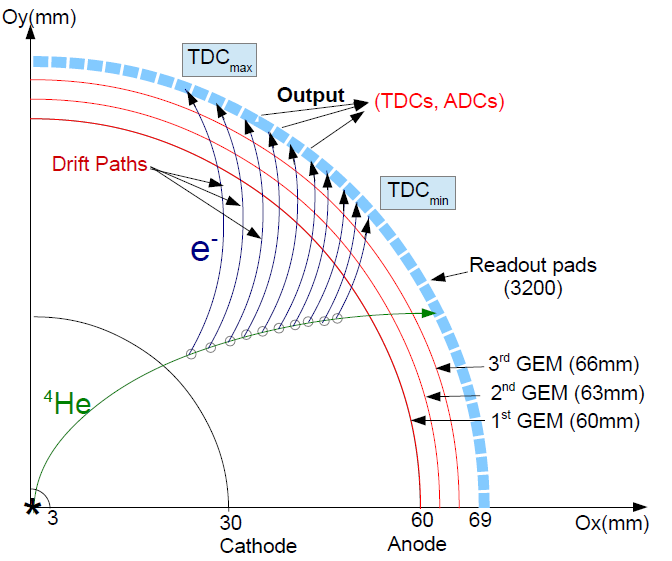
\includegraphics[scale=0.35]{fig/RTPC_2.png}
\caption[]{A schematic drawing of a $^{4}$He track (in green) traversing the 
drift region, with the drift paths followed by the electrons (in black). } 
\label{fig:RTPC_signals}
\end{figure}

To measure the drift speed, we use the time profile of all hits in the 
chamber shown in figure \ref{fig:TDC_profile}. We can clearly observe the 
dropping edge expected from geometrical considerations. We define a value $T_{Max/2}$ at 
which the dropping edge passes half the maximum number of hits in the 
histogram. This value is measure in bins along the 200 mm RTPC's length to take into 
account variations in the electric and magnetic field in the RTPC (see figure 
\ref{fig:RunNumber_61551_TDCmax_Zslice}). 

\begin{figure}[tb]
   \centering
   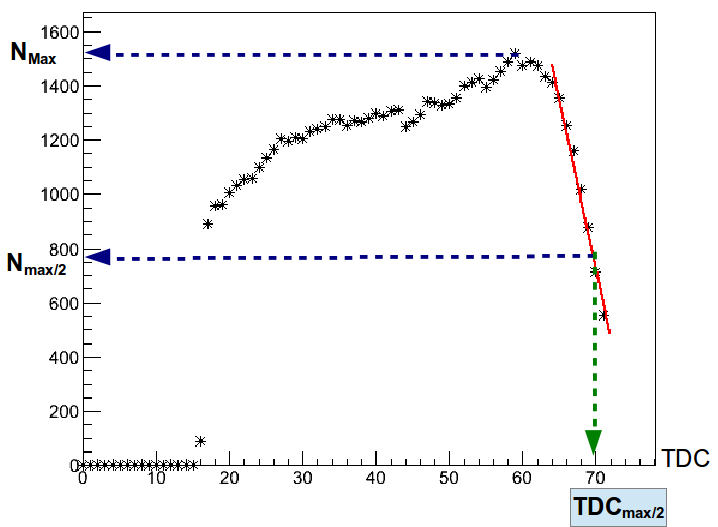
\includegraphics[scale=0.3]{fig/TDC_profile.png}
   \caption[]{Time profile of the collected hits in one experimental run.  } 
   \label{fig:TDC_profile}
\end{figure}

\begin{figure}[tb]
\centering
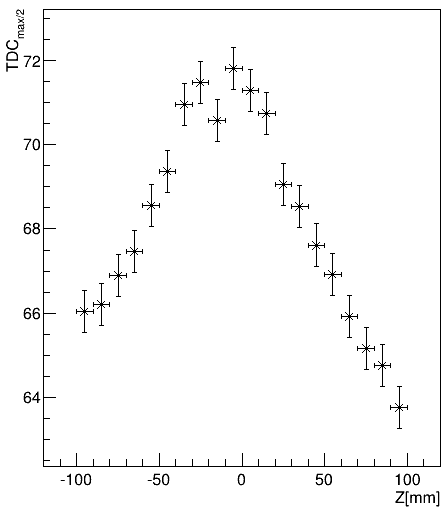
\includegraphics[scale=0.36]{fig/RunNumber_61551_TDCmax_Zslice.png}
\caption{Time profile distribution for the collected hits in one experimental 
run. } \label{fig:RunNumber_61551_TDCmax_Zslice}
\end{figure}

Due to the non perfect experimental conditions, in particular variations in the 
gas mixture\footnote{It was noted during the experiment that leaks appeared
and the gas flow had to be increased in few occasions to compensate for this.}, 
the drift speed changes during the three months long experimental run.  
Figure \ref{fig:Drift_run_number_1} shows the $T_{Max/2}$ values for 
individual runs (approximately 2 hours long). We observe a significant 
variation of the drift speed over time and accounted for it in the drift 
speed used for the track reconstruction. 

In summary, we obtain from our calibration a parametrization of the drift speed 
as a function of both position along the beam axis and run number (we did not 
observe any correlation between the effects). These 
functions were extracted for our entire data set and implemented in the 
track reconstructions code.

\begin{figure}[tb]
\hspace*{-1.8cm}
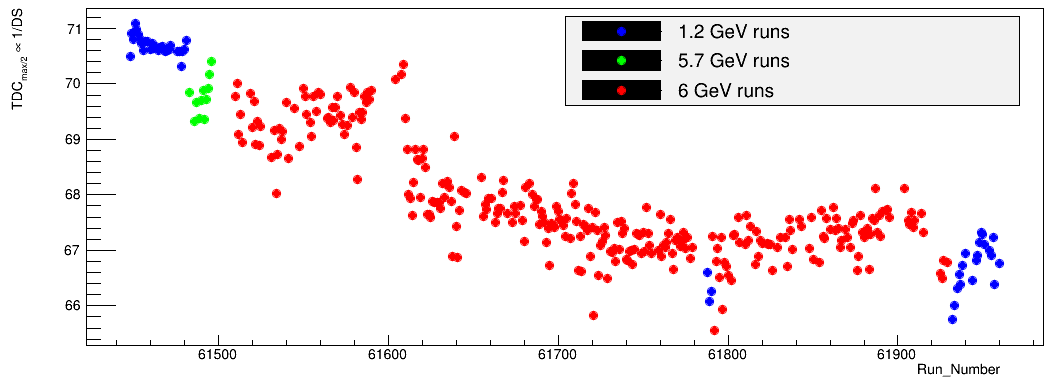
\includegraphics[scale=0.26]{fig/Drift_run_number_1.png}
\caption{$TDC_{Nbmax/2}$ versus the experimental run numbers (time).  } 
\label{fig:Drift_run_number_1}
\end{figure}

   
\subsection{Drift Paths Calibration}

The drift path is the trajectory followed by the electrons released through 
ionization in the gas. Software exists to calculate the drift paths, in particular
MAGBOLTZ~\cite{MAGBOLTZ}, but it requires knowledge of the detector's 
geometry, gas mixture composition, and of course the electric and magnetic 
fields over the whole volume of the detector. We used such calculation as a 
first calibration, but, 
as can be seen with the drift speed, gas composition is far from stable in the 
chamber. Moreover, the 4 $\mu$m foil used as a cathode is easily deformed, such
that we expect the geometry accuracy to be around the millimeter precision. 
These problems, already 
encountered for the BoNuS RTPC calibration~\cite{BONUS-NIM}, motivated the 
acquisition of specific calibration runs. These are taken with a lower energy 
electron beam (1.20 and 1.27 GeV) to enhance the cross section of the elastic 
process ($e^{4}$He$\rightarrow e^{4}$He)
{\bf \color{red} Specify luminosity ?}. In this process, the measurement of
electron kinematics allows to calculate the Helium nucleus kinematic. It is
by comparing this calculated kinematic to the measured one that we fine tune
the drift paths independently of our knowledge of the exact conditions in the 
chamber.

The drift paths are ajusted using a set of identified elastic events 
from our lower beam energy run. Based on the kinematic of the electrons in
these events, we generate the helium nucleus in a GEANT4 
simulation~\cite{GEANT4} of our RTPC. Then we compare the calculated GEANT4 trajectory of 
the Helium nuclei to the hits measured in the chamber. 

Because of the 
magnetic field, the drift paths are not linear in the RTPC. So to perform the extraction, 
we make a first approximation with a linear dependence between the radius of 
emission and the time of detection, and then refine our result. As it happens, 
the curvature is minimal and this process converge already on the second 
iteration. 

At the end of the extraction procedure, where we work in a polar coordinate 
system ($R$,$\phi$), the azimuthal difference between the detection pad and 
the ionization point ($\Delta\phi$) is extracted as a function of time. 
In figure~\ref{fig:DELTA_PHI_TDC}, we show the resulting data points for one 
bin, where the drift paths is easily identified and eventually fitted for 
implementation in our reconstruction codes.

\begin{figure}[tb]
\centering
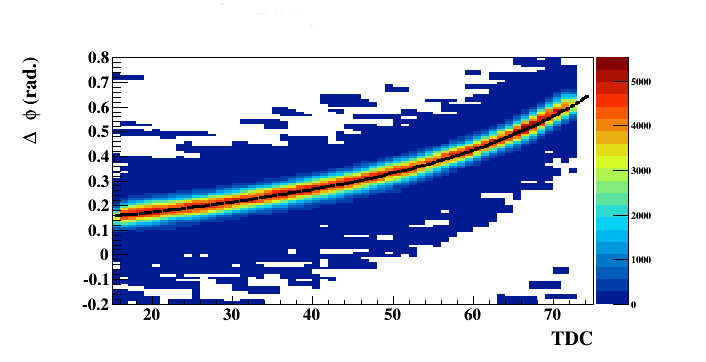
\includegraphics[scale=0.37]{fig/FitResult_p2_10.png}
\caption{$\Delta \phi$ versus TDC distribution in the second pass for tracks
near 35 mm longitudinal position along the RTPC. The black line represents 
the final drift paths in this slice.}
\label{fig:DELTA_PHI_TDC}
\end{figure}

To verify the stability of the drift paths, this procedure was carried out 
using both the 1.204 GeV data from the beginning of the run period and the 
1.269 GeV data from the end of the run period (shown in blue on 
figure~\ref{fig:Drift_run_number_1}). Strangely, we found very similar drift paths
for the two data sets and concluded that any changes in the system only
significantly affected the drift speed.

\subsection{Gain Calibration}

The parametrization of the drift speed and the drift paths were carried out 
using only the TDCs, gain calibration goal is to equalize the gains in ADC/MeV 
over the full RTPC. The gain of each pad is the ratio between the actual 
deposited energy and the registered ADC value. We implemented three different 
methods to extract such gains, with varying degrees of success.

The first method is based on the measured average $\small{\frac{dE}{dX}}$
and the expected value based on the Bethe-Bloch formula (PDG REF).  The total energy
deposition for each $^4$He track is calculated as the sum of all ADC hits
attributed to the track.  The path length of that energy deposition is
calculated as the distance along the reconstructed trajectory between the first
and last hits on the track and corrected to account for regions
of bad channels along the track.  The measured average energy loss is then the
ratio of deposited energy and path length.  The Bethe-Bloch formula is
evaluated at the track's reconstructed momentum, and the ratio with the measured
$\small{\frac{dE}{dX}}$ is taken as a gain scaling factor.  This average gain is
attributed equally to each readout channel contributing to the track, and each
channel's gain is averaged over many tracks.  This gain calibration method is
inherently iterative, and, while it does result in measured $\small{\frac{dE}{dX}}$
much closer to the expected Bethe-Bloch curve than prior to calibration, the
results were not very satisfactory.

The second method is to compare the experimental ADCs to the energy deposited in 
GEANT4 by simulated tracks (using the same elastic events than for the drift 
paths calibration).  This requires a very good GEANT4 simulation 
including drift paths, but also drift and amplification spreads of the charges 
before reaching the pad, so that the simulated hits match the experimental 
ones. Moreover, the simulation has to match the data acquisition (DAQ) features 
that can lead to cutting out hits. After setting the simulation properly, we 
can compare simulation to data on an event by event basis as in 
figure~\ref{fig:EVENT_adc_tdc}. In this step, the gain for each pad is defined 
as the ratio of the measured ADCs to the simulated deposited energy.

In the third method, the ADC value of each pad is compared to 
the ADCs of the other pads inside each track.
(Detail of 3rd method: Mohammad)

Do you want to show $log(dE/dX)$?

\begin{figure}[tb]
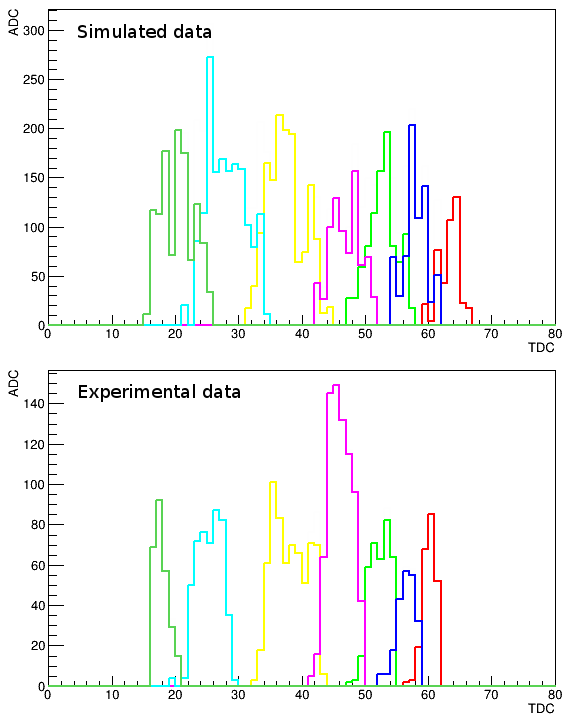
\includegraphics[scale=0.350]{fig/EVENT_adc_tdc.png}
\caption{Simulated (upper) and experimental (lower) ADCs and TDCs distributions 
of a track. The colors indicate the pads, same color in top and bottom indicate 
that they are the same pad.}
\label{fig:EVENT_adc_tdc}
\end{figure}

\begin{figure}[tb]
   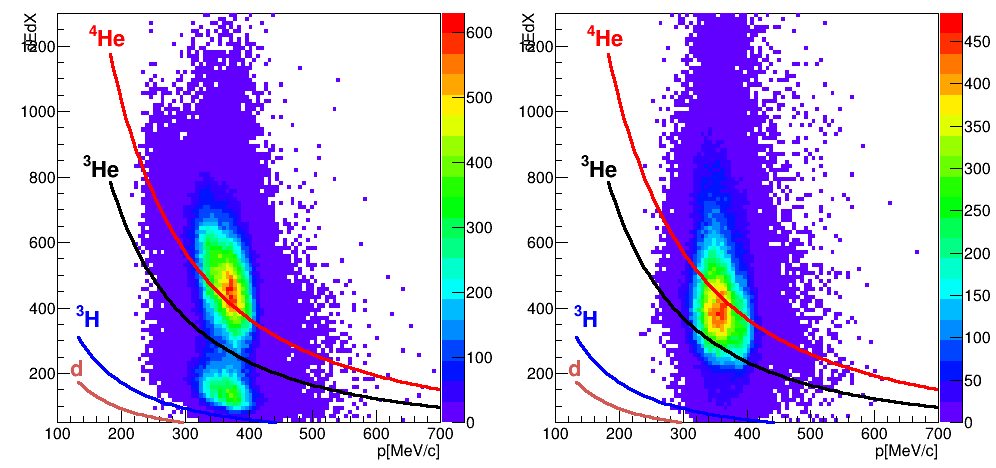
\includegraphics[scale=0.26]{fig/dedx_p_exp_1st.png}
   \caption{$\small{\frac{dE}{dX}}$ vs. p distribution for the left half of the 
      RTPC (left) and for the right half (right). Here, $\small{\frac{dE}{dX}}$ 
   is calculated using the gains of the first method.  The lines are 
theoretical expectations from Bethe-Bloch formula for $^4$He, $^3$He, $^3$H and 
$^2$H (d).}
\label{fig:dedx_p_exp_1st}
\end{figure}

\begin{figure}[tb]
\centering
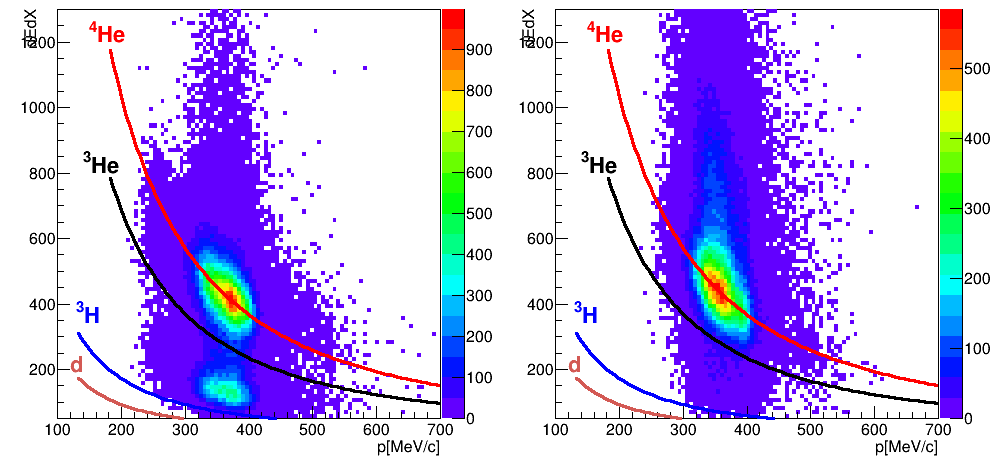
\includegraphics[scale=0.26]{fig/dedx_p_exp_2nd.png}
\caption{$\small{\frac{dE}{dX}}$ vs. p distribution for the left half of the 
   RTPC (left) and for the right half (right). Here, $\small{\frac{dE}{dX}}$ is 
   calculated using the gains of the second method.  The lines are theoretical 
   expectations from Bethe-Bloch formula for $^4$He, $^3$He, $^3$H and $^2$H 
(d).}
\label{fig:dedx_p_exp_2nd}
\end{figure}

A set of gains has been extracted from each method, in 
figure~\ref{fig:dedx_p_exp_1st}, we have $\small{\frac{dE}{dX}}$ calculated 
using the first method's gains, while in Figure~\ref{fig:dedx_p_exp_2nd} we use 
the second method's gains. From these, we concluded that the gains of the 
second method match best the theoretical lines. This is not surprising since 
calibrating with full tracks leads to mixing the gains from the different pads.  
So it seems that even with several iterations, we could not decipher properly 
the effects of individual pads with this method.

\subsection{Noise Rejection}
Two independent noise signatures were identified in the raw data and removed in software prior to track reconstruction.  Both are transient and isolated to a subset of the readout channels. 

The first is an oscillatory noise located early in the readout time window, shown in the top panel of Figure~\ref{fig:noise} for a particularly noisy channel.  Its amplitude is not dissimilar to those of real tracks, and about 18\% of the readout channels exhibit large contributions from this noise characteristic.  Due to its unique time-energy correlation for the given channels, the noise could be removed on an event by event and channel by channel basis without significant loss of good signals, and the result is illustrated in the bottom panel of Figure~\ref{fig:noise}.

The second is a coherent noise affecting about 25\% of the pramplifiers, where the signature is simultaneous hits in most of the 16 channels in a preamp group.   An event-based technique to identify and remove it was developed based on counting simultaneous hits in preamp group, and, if sufficiently large, perform a dynamic pedestal subtraction based on the average ADC of the channels' neighbors within the preamp group.

The sources of these effects were not determined, but rejection techniques allowed to reconstruct 10\% more good tracks, with no significant loss, and recover 70 channels that were previously ignored due to excessive noise levels.

\begin{figure}[tb]\centering
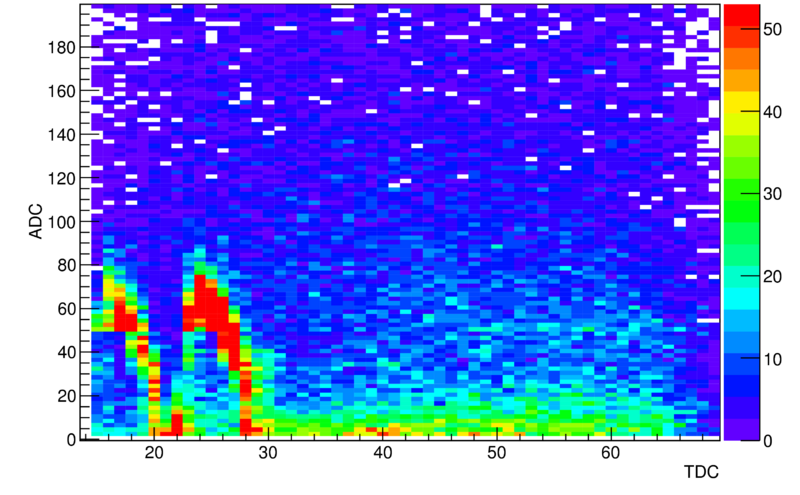
\includegraphics[scale=0.27]{fig/noisy_pad_before_rejection2.png}
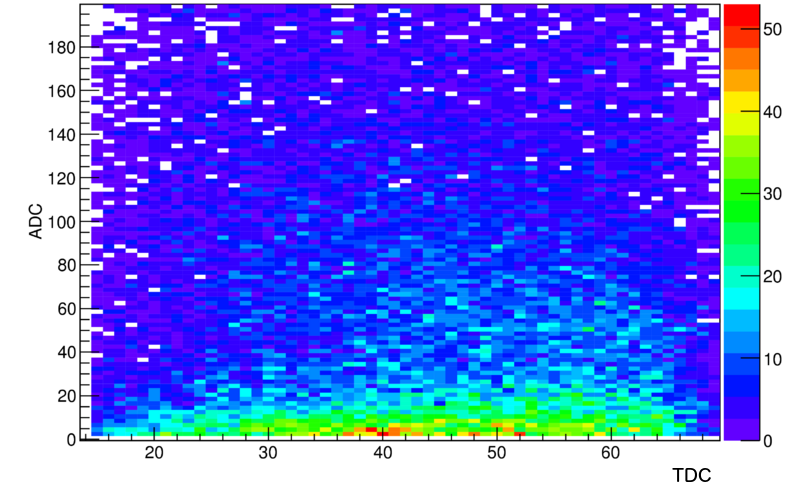
\includegraphics[scale=0.27]{fig/noisy_pad_after_rejection2.png}
\caption{The ADC vs. TDC spectrum for an example noisy channel before (top) and after (bottom) noise rejection algorithms.  Only hits associated with tracks are included, and the selection of events and tracks is the same in both plots.}
\label{fig:noise}
\end{figure}

%\begin{figure}[tb]
%\hspace{-0.4cm}
%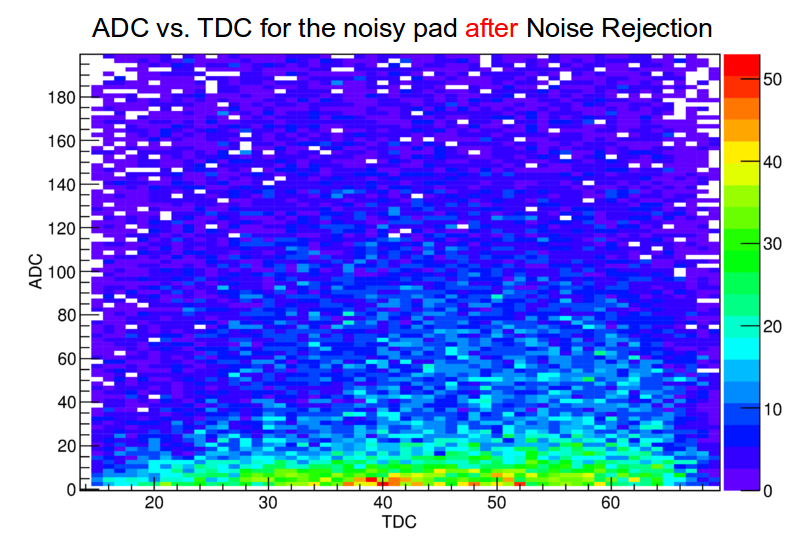
\includegraphics[scale=0.27]{fig/noisy_pad_after_rejection.png}
%\caption{}
%\label{fig:noisy_pad_after_rejection}
%\end{figure}

\section{Track Reconstruction}\label{sec_perf}

In order to reconstruct tracks we first select good hits. This means rejecting 
out-of-time hits and hits linked to the electronic noise. The second step is 
space-reconstructing the hits using the extracted drift speed and drift path 
parameters. For each registered hit, we calculate a position of emission from 
the recorded time (TDC) and the position of the recording pad. The third step 
is to create chains of hits. The maximum distance between two close adjacent 
hits has to be less than 10.5 mm to chain them, this roughly correspond to 
neighbors and next to neighbors. Then, we fit the chains that have a minimum of 
10 hits. We make the fit in two iterations, first, all the hits of the chain 
together with the beam line are fitted with a helix. For the second iteration, 
the hits that are 5 mm or farther from the first fit are excluded.

For energy deposition, the mean $\frac{dE}{dx}$ is calculated as
\begin{equation}
 \left\langle \frac{dE}{dX} \right\rangle= \frac{\sum\limits_{i} \frac{ADC_{i}}{G_i}}{L},
\end{equation}
where the sum runs over all the hits of the track, $G_{i}$ is the gain of 
the associated pad, and $L$ is the visible track length in the active drift 
volume. 

(We need some performance studies here: Mohammad)

\section{Conclusion}




\input acknowledgement.tex  

\begin{thebibliography}{99}

\bibitem{CLASref}
   B.A. Mecking et al., The CEBAF large acceptance spectrometer, Nucl. Inst. 
   and Meth. A 503, 513 (2003).

\bibitem{proposal}
   K.Hafidi et al., Deeply virtual Comton scattering off $^{4}$He, Jlab 
   proposal to PAC33 (2007).

\bibitem{DCref}
   M.D. Mestayer et al., The CLAS drift chamber System, Nucl. Inst.  and Meth.  
   A 449, 81 (2000).

\bibitem{CCref}
   G. Adams et al., The CLAS Cerenkov detector", Nucl. Inst. and Meth. A 465, 
   414 (2001).

\bibitem{TOFref}
   E.S. Smith et al., The time-of-flight system for CLAS, Nucl.  Inst. and 
   Meth. A 432, 265 (1999).

\bibitem{ECref}
   M. Amarian et al., The CLAS forward electromagnetic calorimeter, Nucl.  
   Inst. and Meth. A 460, 239 (2001). 

\bibitem{Hyon-suk}
   Hyon-Suk Jo, Etude de la Diffusion Compton Profond{\'e}ment Virtuelle Sur le 
   Nucl{\'e}on avec le D{\'e}tecteur CLAS de Jefferson Lab: Mesure des Sections 
   Efficaces polaris{\'e}es et non polaris{\'e}es, IPNO-Thesis, 2007.

\bibitem{gem_sauli}
   F. Sauli, GEM: A new concept for electron amplification in gas detectors, 
   Nucl. Instr. and Meth. A 386, 531 (1997).

\bibitem{BONUS}
   S. Tkachenko et al., Measurement of the nearly free neutron structure 
   function using spectator tagging in inelastic $^{2}H(e,e'p)X$ scattering 
   with CLAS,	Phys. Rev. C 89, 045206 (2014).

\bibitem{MAGBOLTZ}
   S. Biagi, Monte Carlo simulation of electron drift and diffusion in counting 
   gases under the influence of electric and magnetic fields, Nucl.  Inst. and 
   Meth. in Phy. Res. A, vol. 421, pp. 234-240, 1999.

\bibitem{GEANT4}
http://geant4.cern.ch
 	
\bibitem{BONUS-NIM}
Howard C. Fenker et al., BoNuS: Development and Use of a Radial TPC using Cylindrical GEMs, Nucl. Instrum. Meth. A592, 273-286 (2008)
\end{thebibliography}

\end{document}

